\begin{question}[topic=gsm,name={15.06.2016},type=exam,tags={20160615}]
Eine kompensierte \textbf{Nebenschluss-Gleichstrommaschine} hat folgende Daten. Eine Leerlaufkennlinie \textbf{$U_i=f(I_E)$ bei $n=1000~U/min$} ist gegeben (siehe Abb.\ref{fig:20160615}).\\
\begin{tabular}{L{2cm}l}
$I_{A,N}$ \dotfill &$200~A$\\
$U_{A,N}$ \dotfill & $40~V$ \\
$n_N$ \dotfill & $2000~\frac{U}{min}$
\end{tabular}
\begin{enumerate}
\item Skizzieren Sie die Schaltung der Nebenschlussmaschine am Gleichspannungsnetz. (\addpoints{1})
\item Wie groß ist bei Nennspannung $U_{A,N}$ im motorischen Betrieb die Spannungskonstante $k_1 \phi_N$ im Nennpunkt, das Nennmoment $M_N$ und die mechanische Nennleistung $P_N$ der Gleichstrommaschine, wenn ein Erregerwiderstand $R_E=2,5~\Omega$ verwendet wird? (\addpoints{3})
\item Wie groß ist dabei die Leerlaufdrehzahl $n_0$ bei Nennspannung $U_{A,N}$ und wie groß ist der Ankerwiderstand $R_A$ (\addpoints{2})
\item Berechnen Sie den Wirkungsgrad $\eta_N$ im Nennpunkt der Maschine unter Berücksichtigung des Ankerwiderstand $R_A$ und des Erregerwiderstands $R_E = 2,5~\Omega$. Die mechanischen Verluste, Bürstenverluste und Eisenverluste werden vernachlässigt. (\addpoints{1})
\item Die Maschine wird bei einer konstanten Drehzahl $n=2000~U/min$ \underline{als Generator} mit $R_E =2,5~\Omega$ eingesetzt und mit einem umschaltbaren Lastwiderstand $R_L = 0,01\, /\, 0,02\, /\, 0,05 ~\Omega$ belastet. Berechnen Sie jeweils den Laststrom und den Erregerstrom und skizzieren Sie die (äussere) Generatorkennlinie $U_A=f(I_L)$ für die unterschiedlichen Belastungen inklusive Leerlauf des Generators mit $I_L = 0$. (\addpoints{3})
\end{enumerate}
\begin{figure}[H]
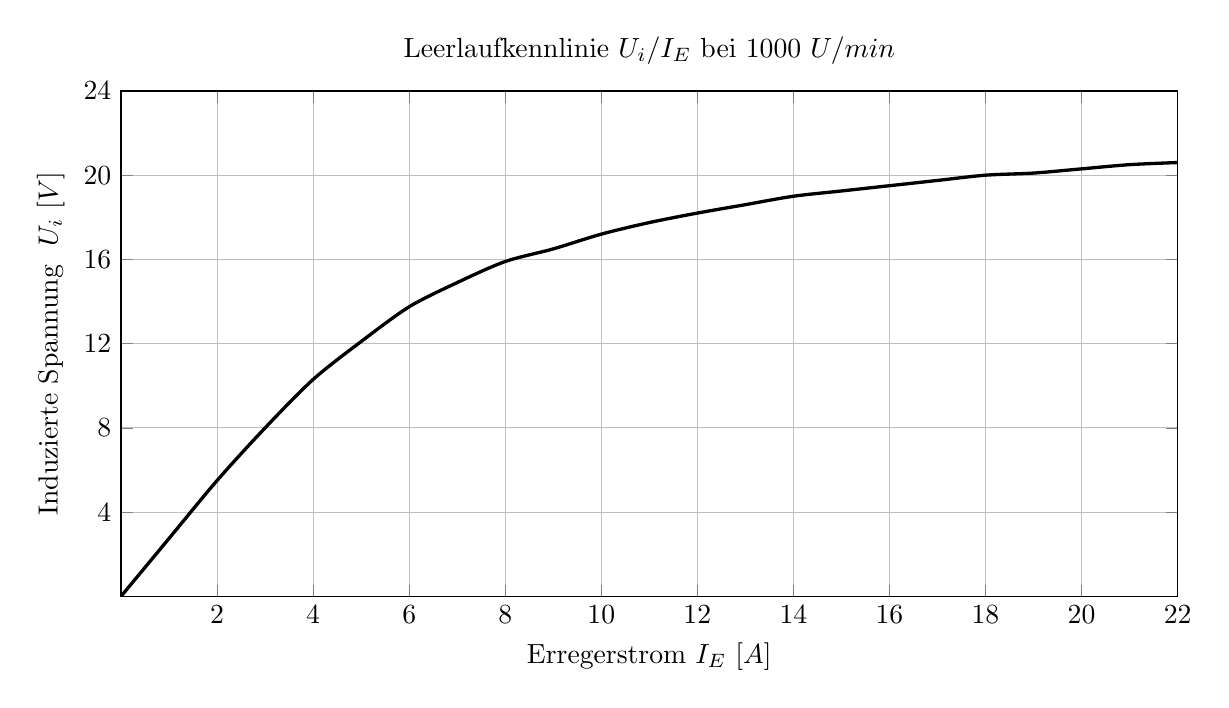
\begin{tikzpicture}
\begin{axis}[title={{Leerlaufkennlinie} $U_i/I_E$ {bei} $1000 ~U/min$},xlabel={{Erregerstrom }$I_E \, \left[A\right]$ }, ylabel={{Induzierte Spannung } $U_i \, \left [V\right]$},
xtick= {2,4,6,8,10,12,14,16,18,20,22},width=15cm,height=8cm,
xmin = 0,xmax = 22,
ytick= {4,8,12,16,20,24},
ymin = 0 , ymax = 24,grid=major]
\addplot+
[id=exp,color=black,mark=none,smooth, very thick] coordinates {
	( 0,0)
	(1,2.75)
	(2,5.5)
	(3,8)
	(4,10.3)
	(5,12.1)
	(6,13.75)
	(7,14.9)
	(8,15.9)
	(9,16.5)
	(10,17.2)
	(11,17.75)
	(12,18.2)
	(13,18.6)
	(14,19)
	(15,19.25)
	(16,19.5)
	(17,19.75)
	(18,20)
	(19,20.1)
	(20,20.3)
	(21,20.5)
	(22,20.6)
};
\end{axis}
\end{tikzpicture}
\caption{Leerlaufkennlinie} \label{fig:20160615}
\end{figure}
\end{question}
\begin{solution}
\begin{enumerate}
\item Kann hier jemand mit TikZ die Schaltung programmieren und hier reinstellen?
\item Die Spannungskonstante im Nennpunkt errechnet sich über Glg.(\ref{glg:induziertespannung}). Dazu wird über das Diagramm die Induzierte Spannung bei $I_E$ abgelesen. Einsetzen und auf $k^{'}\Phi$ umformen.
\begin{align}
I_E &= \frac{U_{A,N}}{R_E}=\frac{40}{2,5} = 16~A\\
\Omega_{1000}&= \frac{1000 \cdot 2 \pi}{60} = 104,71~ 1/s\\
\Omega_N&= \frac{2000 \cdot 2 \pi}{60} = 209,43~ 1/s\\
k^{'}\Phi &= \frac{U_i}{\Omega_{1000}} = \frac{19,5V}{104,71}=0,186 ~Vs\\
k_1 \phi_N &= k^{'}\Phi \cdot 2 \pi = 1,17~Vs\\
M_N&=k^{'}\Phi \cdot I_A =0,186 \cdot 200 = 37,242 ~Nm \\
P_N &= M_N \cdot \Omega_N = 37,242 \cdot 209,43 = 7,8 ~kW\\
\end{align}
\item Der Ankerwiderstand errechnet sich über Glg.(\ref{glg:Ankerspannungsgleichung}).
\begin{align}
U_{A,N} & = k^{'}\phi_N \cdot \Omega_0 = k^{'}\phi_N \cdot \frac{n_0}{60} \cdot 2 \pi \\
n_0 & = \frac{U_{A,N} \cdot 60}{k^{'}\phi_N \cdot 2 \pi} = \frac{40 \cdot 60}{0,186 \cdot 2 \pi} = 2053,61 ~U/min\\
\Omega_0 &= \frac{n_0 \cdot 2 \pi}{60} = \frac{2053,61 \cdot 2 \pi}{60}=215,05~1/s\\
R_A &= \frac{k^{'}\phi_N \cdot (\Omega_0 -\Omega_N)}{I_N} =\frac{0,186 \cdot (215,05 -209,43)}{200} = 5,22~m\Omega
\end{align}
\item Der Wirkungsgrad errechnet sich über Glg.(\ref{glg:Wirkungsgrad}). Hier müssen aber die Verluste über die Erregerwicklung berückischtigt werden.
\begin{equation}
\eta_N = \frac{M_N \cdot \Omega_N}{U_N \cdot (I_N+ I_E)} = \frac{37,242 Nm \cdot 209,43 1/s}{40 \cdot (200 + 16)}=0,903
\end{equation}
\item Hier bitte ein Bild von der Schaltung. Der Strom $I_A$ ist jetzt negativ, weil wir uns im Generatorbetrieb befinden. Als Startgleichung wird hier Glg.(\ref{glg:Ankerspannungsgleichung}) verwendet. Die Glg wird auf eine Form $U_i(I_E)/I_E$ umgeformt, was einer Steigung entspricht, und dann der Schnittpunkt mit der Linie im Diagramm abgelesen. Da die Drehzahl im Diagramm bei $1000 ~U/min$ aufgenommen wurde, wir aber mit $2000~U/min$ arbeiten, ist für die induzierte Spannung ein Faktor $2$ vorzusehen.
\begin{align}
I_A \cdot R_A + I_L \cdot R_L &= k^{'} \Phi \cdot \frac{2000}{60} \cdot 2 \pi\\
(I_L + I_E) R_A + I_E \cdot R_E &= U_i(I_E) \cdot 2\\
\left (\frac{I_E \cdot R_E}{R_L} + I_E \right )R_A + I_E R_E &= U_i(I_E)\cdot 2\\
R_A I_E \left ( \frac{R_E}{R_L} + 1 \right ) + I_E R_E &= U_i(I_E)\cdot 2\\
I_E\left(R_E +R_A\left(1 + \frac{R_E}{R_L}\right )\right) &= U_i(I_E)\cdot 2\\
\frac{U_i(I_E)}{I_E} &= \frac{R_E +R_A\left(1 + \frac{R_E}{R_L}\right)}{2}\\
\frac{U_i(I_E)}{I_E}|_{R_L=0,01} &= 1,91\\
\frac{U_i(I_E)}{I_E}|_{R_L=0,02} &= 1,58\\
\frac{U_i(I_E)}{I_E}|_{R_L=0,05} &= 1,38\\
\frac{U_i(I_E)}{I_E}|_{R_L=\infty} &= 1,25
\end{align}
Die Steigungen werden in Abb.\ref{fig:20160615} eingezeichnet und bei dem Schnittpunkt mit der Kurve der Erregerstrom und die induzierte Spannung abgelesen. Der Laststrom und die Lastspannung ergeben sich wie folgt:
\begin{align}
I_L &= \frac{I_E \cdot R_E}{R_L}\\
U_L &= I_E \cdot R_E
\end{align}
\begin{tabular}{lcccc}
$R_L$   & $I_E~[A]$  & $U_i~[V]$ & $I_L~[A]$ & $U_L~[V]$\\
$0,01$  & $2$    & $4$   & $500$ & $5$\\
$0,02$  & $8$    & $16$  & $1000$& $20$\\
$0,05$  & $12$   & $18$  & $600$ & $30$\\
$\infty$& $14$   & $19$  & $0$   & $19$\\
\end{tabular}
\begin{figure}[H]
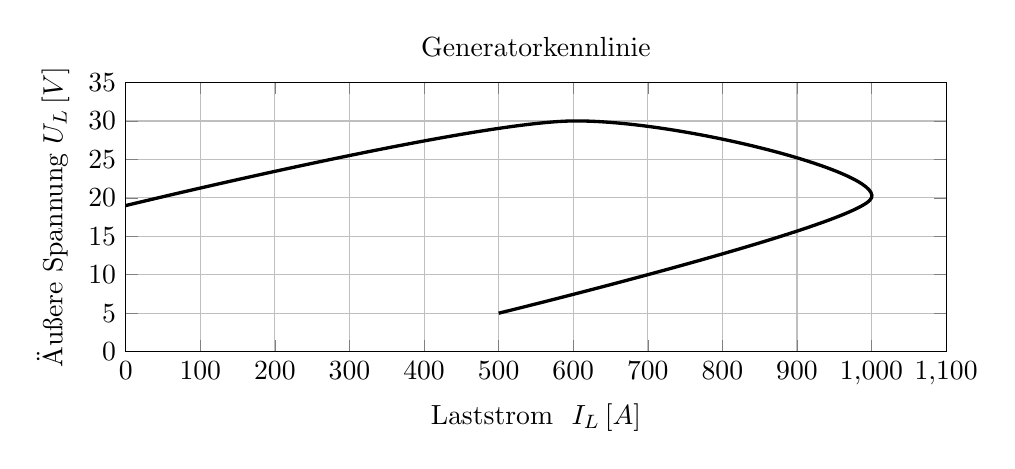
\begin{tikzpicture}
\begin{axis}[title={Generatorkennlinie},xlabel={{Laststrom } $I_L\left [ A \right ]$}, ylabel={{Äußere Spannung }$U_L\left [ V \right ]$ },
xtick= { 0,100,...,1100},width=12cm,height=5cm,
xmin = 0,xmax = 1100,
ytick= {0,5,...,35},
ymin = 0 , ymax = 35,grid=major]
\addplot [black,no marks,very thick,smooth ]coordinates {
	(500,5)
	(1000,20) 
	(600,30) 
	(0,19) };
	\end{axis}
	\end{tikzpicture}
	\label{fig:20160615lsg25}
	\end{figure}
	\end{enumerate}
\end{solution}